\documentclass[tikz]{standalone}
\usepackage{tikz}
\usetikzlibrary{positioning, graphs}
\usetikzlibrary{graphs.standard}
\begin{document}
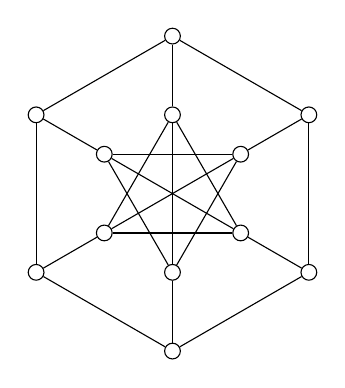
\begin{tikzpicture}
		[every node/.style={draw,circle,inner sep = 0mm, minimum size = 2mm}]
		\graph[clockwise, radius = 2cm, empty nodes]{subgraph C_n[n = 6, name = A]};
		\graph[clockwise, radius = 1cm, empty nodes] {subgraph I_n [n = 6, name = B]};
		\foreach \i [evaluate={\j=int(mod(\i+1,6)+1);\k=int(mod(\i+2,3)+1)}] in {1,...,6}{
		\draw (A \i) -- (B \i);
		\draw (B \i) -- (B \j);
		\draw (B \i) -- (B \k);
		}
\end{tikzpicture}
\end{document}